\documentclass[a4paper,12pt]{report}
\usepackage[T1]{fontenc}
\usepackage[utf8]{inputenc}
\def\magyarOptions{defaults=hu-min}
\usepackage[magyar]{babel}
\usepackage{amsthm, amssymb, amsmath,hyperref}
\usepackage{enumerate, graphicx, xcolor}

\usepackage{chngcntr}
\counterwithout{figure}{chapter}
\counterwithout{figure}{section}
\counterwithout{figure}{subsection}
%\usepackage{pgf,tikz,float}
%\usepackage{tikzlings}
%\usepackage{tikzducks}
%\usetikzlibrary{arrows}
\usepackage[nobysame]{amsrefs}
%\usepackage{amsmath}

\usepackage{geometry}
   \geometry{
   a4paper,
   total={160mm,247mm},
   left=25mm,
   top=25mm,
}

\date{today}
\linespread{1.3}
\tolerance 8000
\hbadness 8000


\begin{document}
\thispagestyle{empty}

\begin{center}
\vspace*{0.2cm} {\Large\bf Szegedi Tudományegyetem}
\vspace{0.3cm}

{\Large\bf Természettudományi és Informatikai Kar}
\vspace{0.3cm}

{\Large\bf Informatikai Intézet, Számítástudomány Alapjai Tanszék}
\vspace{3cm}

{\Large SZAKDOLGOZAT}

\vspace*{1.5cm}

{\LARGE\bf Tanulmányokat segítő webalkalmazás egyetemi hallgatók számára}

\vspace*{4cm}

{\large
    \begin{tabular}{c@{\hspace{2cm}}c}
        \emph{Készítette:} &\emph{Külső témavezető:}\\
        \bf{Kozma Kristóf} &\bf{Dr. Iván Szabolcs}\\
        Programtervező Informatikus & Szoftverfejlesztő\\
        BSc hallgató & HighTec Hungary Kft.\\
        & \\
        & \emph{Belső konzulens:}\\
        & \bf{Dr. Gazdag Zsolt}\\
        & Egyetemi docens
    \end{tabular}
}

\vspace*{1,5cm}

{\Large Szeged\\ \vspace{2mm} 2024}
\end{center}


\newpage
{\Huge \bf Feladatkiírás}

\vspace{2 cm}

Az egyetemi hallgatóknak rengeteg információval kell tisztában lenniük. Látniuk kell a mintatantervbeli haladásukat, a tanulmányai átlagukat különböző ösztöndíjak tekintetében, és meg kell tervezniük az időbeosztásukat az egyetemi órák mellett, hiszen sokan ekkor kezdenek el dolgozni is. A hallgató feladata egy webalkalmazás létrehozása, ami képes könnyűvé és gördülékennyé tenni ezeket a folyamatokat, valamint átláthatóan rendszerezni a hallgatók számára fontos, az egyetemmel kapcsolatos általános tudnivalókat.


\newpage
{\Huge \bf Tartalmi összefoglaló}

\vspace{2 cm}

Dolgozatom témája egy tanulmányokat segítő webalkalmazás elkészítése egyetemi hallgatók számára. Célom egy olyan alkalmazás elkészítése volt, mely nagyban meg tudja könnyíteni az egyetemi hallgatók számára tanulmányaik követését mindennapjaik során. Ehhez az Angular nevű TypeScript keretrendszert választottam, mert ideálisnak tartom nagy alkalmazások elkészítéséhez, melyek sok, jól elkülöníthető részre tagozódnak, és összetett adatfolyamokkal dolgoznak. Ezen kívül hangsúlyt fektettem rá, hogy ne csak a Szegedi Tudományegyetem hallgatóira szabjam az alkalmazást, hanem általánossá tegyem, hogy akár az egész országban használható legyen egyetemi hallgatók számára.

Az elkészült Apollo nevű alkalmazás véleményem szerint sikeresen kielégíti ezeket az igényeket, és több egyetemi hallgató ismerősöm is megerősítette ezt.

\vspace{1 cm}

\textbf{Kulcsszavak}: webalkalmazás, tanulmányi rendszer, felsőoktatás, hallgató, Angular


\newpage
\pagebreak

\tableofcontents
\pagebreak

\chapter{Bevezetés}

\section{Motiváció}

Egyetemi tanulmányaim során én is sokszor éreztem azt a problémát, hogy nem tudom, hogy állok a mintatantervben, mert a Neptun \cite{neptun} és a CooSpace \cite{coospace} rendszerében nagyon nehezen elérhetők az ezzel kapcsolatos információk, és magukat a közzétett adatokat sem könnyű átlátni. Ezenkívül sokszor Excel táblában számoltam vizsgaidőszakban az átlagomat, akár tanulmányi ösztöndíjjal kapcsolatban, mert erre nem nyílt egyszerűbb mód. Valamint az órarend megtervezését is mindig nehézségnek éreztem, amikor össze kellett állítanom a sok lehetséges kurzus közül, hogy melyikeket szeretném felvenni. Ezeket a problémákat szerettem volna megoldani, amik bármelyik hallgató tanulmányai során felmerülhetnek.

\section{Az alkalmazás neve}

Az alkalmazásnak az Apollo nevet adtam. A Neptunhoz hasonlóan egy ókori istenről szerettem volna elnevezni. Azért Apollónra esett a választásom, mert bár legszélesebb körben a Nap, a művészetek és az íjászat isteneként ismert, ő a tudás, oktatás és fiatalság istene, valamint a zenéé és a táncé is, amik nagyon jól kapcsolódnak az egyetemistákhoz. Ezzel szerettem volna jelezni, hogy az alkalmazás az egyetemi hallgatók hétköznapjainak megkönnyítésére készült.

\section{Elérhetőség}

Az alkalmazásnak a forráskódja elérhető saját GitHub oldalamon a \url{https://github.com/bechryko/szakdolgozat-apollo} címen.

\chapter{Az alkalmazás megtervezése}

\section{Terület áttekintése}

A kiinduláshoz figyelembe vettem, hogy milyen alkalmazások/weboldalak érhetőek el a magyar egyetemisták számára, amik ki tudják elégíteni a bennem is felmerült igényeket, valamint felhasználói interjúkat készítettem, hogy mások, más nézőpontból is rá tudjanak világítani ezekre a nehézségekre, és képet kapjak több felhasználó igényeiről is.

\subsection{Piackutatás}

Magyarország legnagyobb egyetemi tanulmányi alkalmazása a Neptun, melyben elérhetők azok a funkciók, melyeket az Apollo is szeretne megvalósítani, csak véleményem szerint egyik sem eléggé felhasználóbarát módon:

\begin{itemize}
    \item A mintatantervbeli haladás megtekintésére nincs mód, egyedül a teljes mintatantervet lehet megtekinteni, és azzal egyesével összehasonlítani a hallgató által már elvégzett vagy elvégzendő kurzusokat. Ugyanez a helyzet a specializációkkal is, a Neptun felülete ugyanúgy teszi lehetővé a specializációkkal való haladás megtekintését, mint a mintatantervét.
    \item A tanulmányi átlagokat megjeleníti a Neptun, azonban a hallgatónak nincs lehetősége, hogy tudjon ezekkel tervezni is. Leginkább vizsgaidőszakban releváns a hallgatók számára az átlaguk, amikor megtervezik, melyik vizsgára mennyit készüljenek, a Neptun azonban csak a vizsgaidőszak lezártával teszi láthatóvá az átlagokat, ami megakadályozza a hallgatókat, hogy a tervezéshez fel tudják használni a Neptun átlagösszesítő funkcióját.
    \item A Neptunban van órarendtervező funkció, amivel az adott tárgyhoz kötődő egyetlen kurzust hozzá lehet adni az órarendhez, ami képes lehet vizualizálni az esetleges óraütközéseket. Azonban egy nagyobb létszámú szakon, például programtervező informatikus BSc szakon, ahol egyetlen tárgyhoz akár tíz gyakorlat is meg lehet hirdetve, nagyon nehéz eldönteni ez alapján, hogy a hallgatónak melyik a legmegfelelőbb a felsorolt órák közül. Továbbá, ha figyelembe akarja venni az egyéb, egyetemen kívüli elfoglaltságait (munka, sport, rendszeres közösségi programokra járás), azt már meg sem teheti a Neptunban, csak egy külső naptár alkalmazás segítségével.
    \item A Neptun teremkereső funkciója a legtöbb hallgató számára rejtély, sokan nem is tudják, hogy létezik, mert egy sokadik almenüpontban található a Neptunon belül. A felülete maga nem túl informatív, hiszen csak egyetlen teremre lehet rákeresni, és azt sem mutatja meg egy térképen, hanem át kell navigálni a Google Térképre, hogy ott meg lehessen tekinteni, hogy az a város mely részén van.
    \item A legnagyobb előnye a Neptunnak, hogy minden hivatalos adat megtalálható rajta, ami a hallgatóhoz kapcsolódik. A Neptun hatalmas mennyiségű adattal dolgozik (például egy egyetemen több ezer tantárgy van), és ezeknek az adatoknak az átmozgatása bármilyen más alkalmazásba komoly nehézségeket jelenthet.
\end{itemize}

\subsection{Felhasználói interjúk}

A felhasználói interjúk során a következő problémákat véltem felfedezni, amiben más egyetemisták is szenvednek a Neptun használata során:

\begin{itemize}
    \item Az átlagok azonnali kiszámítása fontos lenne vizsgaidőszakban. Nagyon sokan számolják egy Excel táblázatban az átlagukat, vagy akár tantárgyanként a pontszámaikat, amivel képet kaphatnak körülbelül az elkövetkező félév végi eredményeikről.
    \item A tanulmányi vagy állami ösztöndíjak feltételei sokak számára nem világosak, és aki szeretné ezeket megkapni, és a ponthatáron van, annak szüksége lenne egy megbízható eszközre, amire hagyatkozhat a jegyeinek a kialakításakor.
    \item A mintatantervbeli haladás követése mindenkinek problémát okoz, sokan ellentmondásos információkkal is találkoznak különböző platformokon, amik alapján nehéz eldönteni, hogy pontosan hol is tartanak a diplomájuk megszerzésében.
    \item Volt, aki azt hozta fel, hogy az egyetemi szabályzat elemei, például a TVSZ egy olyan dolog, amire sokszor hivatkoznak, de annál kevesebben ismerik a pontos tartalmát. Ilyesféle szabályok és az egyetemmel kapcsolatos hasznos információmorzsák megjelenítését is szívesen fogadná egy efféle alkalmazásban.
    \item Többen érdeklődtek egy tanteremkereső funkció iránt, aminek a segítségével az elsőéves hallgatók könnyen megtalálhatják a termeiket az ismeretlen épületekben, de akár abban is segíthet, hogy szabadon használható tanulóhelyeket találjanak a városban, ahol akár egy kávét is elfogyaszthatnak tanulás közben.
\end{itemize}

\section{Funkcionális specifikáció}

\subsection{Funkciólista}

A saját magam és az interjúalanyaim által megfogalmazott problémafelvetések alapján a következő főbb funkciókat vizualizáltam az alkalmazásnak:

\begin{enumerate}
    \item tanulmányi átlagok áttekintése
    \begin{enumerate}
        \item félévek hozzáadása, törlése, módosítása,
        \item jegyek hozzáadása, törlése, módosítása,
        \item jegyek importálása a Neptunból,
        \item átlagok megtekintése (súlyozott átlag, kreditek, kreditindex, korrigált kreditindex),
        \item alternatív jegyek beállítása (például hogyan változna az átlag egy vizsga javítása után),
        \item tanulmányi ösztöndíj számítás (az adott átlaghoz körülbelül milyen ösztöndíj járna az adott szakon),
        \item állami ösztöndíj feltételek teljesülésének jelzése,
        \item vendég felhasználó is felviheti a jegyeit, ami helyileg kerül eltárolásra,
        \item vendég felhasználó törölheti a lokálisan eltárolt adatokat,
    \end{enumerate}
    \item mintatantervbeli haladás áttekintése
    \begin{enumerate}
        \item félévek hozzáadása, törlése, módosítása,
        \item teljesített tárgyak hozzáadása, törlése, módosítása,
        \item tárgycsoportok megtekintése, ahol még hiányzik kredit,
        \item teljesítetlen tárgycsoportok teljesítetlen tárgyainak kilistázása,
        \item specializációk teljesítésének áttekintése,
    \end{enumerate}
    \item órarendtervezés
    \begin{enumerate}
        \item félévek hozzáadása, törlése, módosítása,
        \item kategóriák felvitele, törlése, módosítása, órák hozzáadása kategóriákhoz,
        \item órák felvitele, törlése, módosítása,
        \item órarend megtekintése,
        \item vendég felhasználó is felviheti az óráit, ami helyileg kerül eltárolásra,
        \item vendég felhasználó törölheti a lokálisan eltárolt adatokat,
    \end{enumerate}
    \item autentikáció
    \begin{enumerate}
        \item vendég felhasználó tud regisztrálni és bejelentkezni,
        \item bejelentkezett felhasználó tudja módosítani az adatait és a beállításait,
    \end{enumerate}
    \item adminisztráció: csak admin felhasználók számára
    \begin{enumerate}
        \item egyetemek hozzáadása, módosítása,
        \item egyetemi karok hozzáadása, törlése, módosítása,
        \item tárgyak hozzáadása adott egyetemhez, majd ezek módosítása, törlése,
        \item szakok hozzáadása adott egyetemhez, majd ezek módosítása, törlése,
        \item tárgyak és tantervek importálása a Neptunból,
        \item tárgyak hozzárendelése adott szakhoz, majd ezek módosítása, törlése,
        \item specializációk hozzáadása adott egyetemhez, majd ezek módosítása, törlése,
        \item tárgyak hozzárendelése adott specializációhoz, majd ezek módosítása, törlése,
        \item korábbi évek ösztöndíjértékeinek hozzáadása adott szakhoz, majd ezek módosítása, törlése,
    \end{enumerate}
    \item nyelv átállítása.
\end{enumerate}

\subsection{Folyamatábra}

Egy folyamatábra segítségével terveztem meg az alkalmazás oldalait, és hogy hogyan érhetők el rajta a különböző, az előző pontban megfogalmazott funkciók. Szerettem volna egy letisztult felhasználói élményt nyújtani, ami mégis képes biztosítani a felsorolt funkciókat. Ezt azzal próbáltam elérni, hogy igyekeztem nem sok aloldalt létrehozni, inkább egy oldalon több szekcióban, valamint dialógusablakokban helyeztem el a különböző funkciókat.

Teljesen oválisan jelöltem magukat az oldalakat, valamint szaggatott szegélyt adtam a dialógusablakokban elérhető funkcióknak. Nyíllal jelöltem, amikor felhasználói interakcióval érhető el akár egy oldal (navigálás), akár egy funkció (például egy menü lenyitása).

\Az{\ref{fig:UserFlowchart}.} ábrán az alap felhasználók, \az{\ref{fig:AdminFlowchart}.} ábrán pedig az adminisztrátor felhasználók folyamatábrája látható. Utóbbin csak azokat a funkcionalitásokat tüntettem fel, amik az első, általánosabb ábrán nincsenek rajta.

\begin{figure}
    \centering
    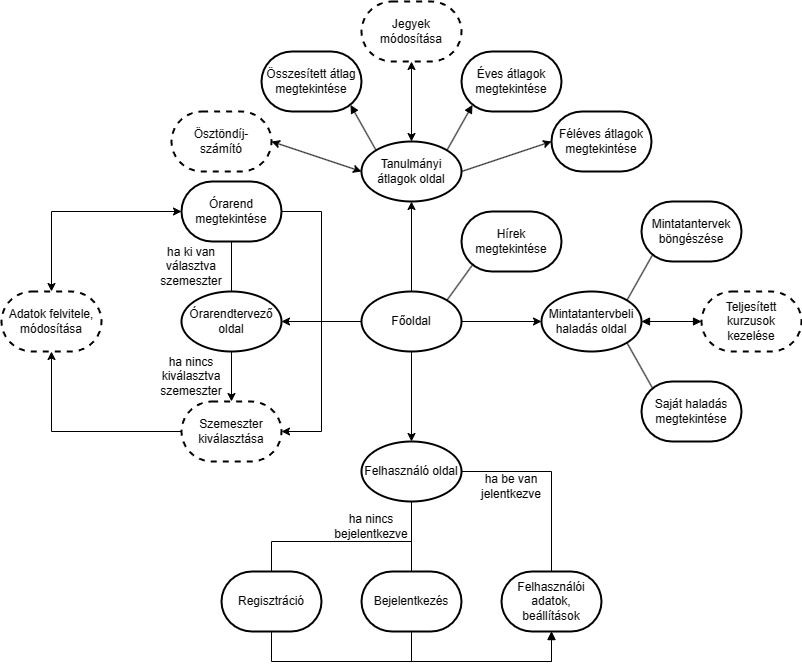
\includegraphics[width=0.8\linewidth]{folyamatábra.png}
    \caption{Az alap felhasználók folyamatábrája \cite{drawio}}
    \label{fig:UserFlowchart}
\end{figure}

\begin{figure}
    \centering
    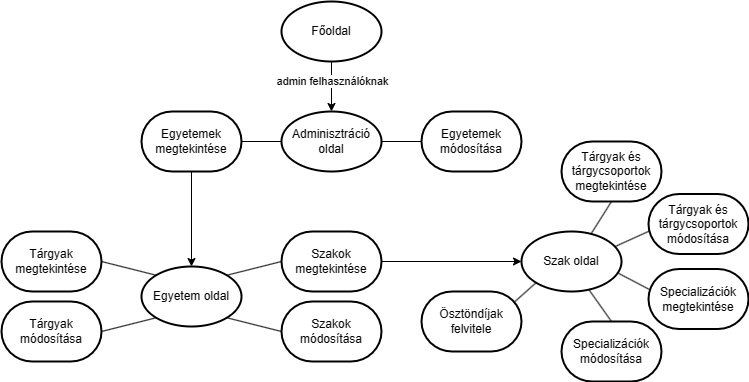
\includegraphics[width=0.75\linewidth]{folyamatábra_admin.png}
    \caption{Az adminisztrátor felhasználók folyamatábrája (kiegészítés az alap folyamatokhoz)}
    \label{fig:AdminFlowchart}
\end{figure}

\section{Vizuális tervezés}

Nagy hangsúlyt fektettem az alkalmazás vizuális tervezésére, hiszen ettől nagyban függ a felhasználói élmény.

\subsection{Hangulattábla (moodboard)}

A hangulattábla \cite{figma-moodboard} a designer-ek egyik eszköze, amivel az alkalmazás vizuális tervezésének egy hangulati alapot állítanak. A hangulattábla hivatott átadni azt a színvilágot, azt az érzést, aminek a felhasználót hatalmába kell kerítenie, amikor az alkalmazást használja és nézi. Szokás elhelyezni rajta példákat hasonló felületekre, színpalettákat, mintákat, formákat és betűtípusokat.

Többször is újraterveztem az alkalmazás hangulattábláját, mert nem voltam elégedett az első változatokkal. Mindenképpen szerettem volna, ha Apollón istenhez is kötődik az alkalmazás színvilága, valamint a meleg színekkel kellemesebb, otthonosabb felhasználói élményt biztosít.

\begin{figure}
    \centering
    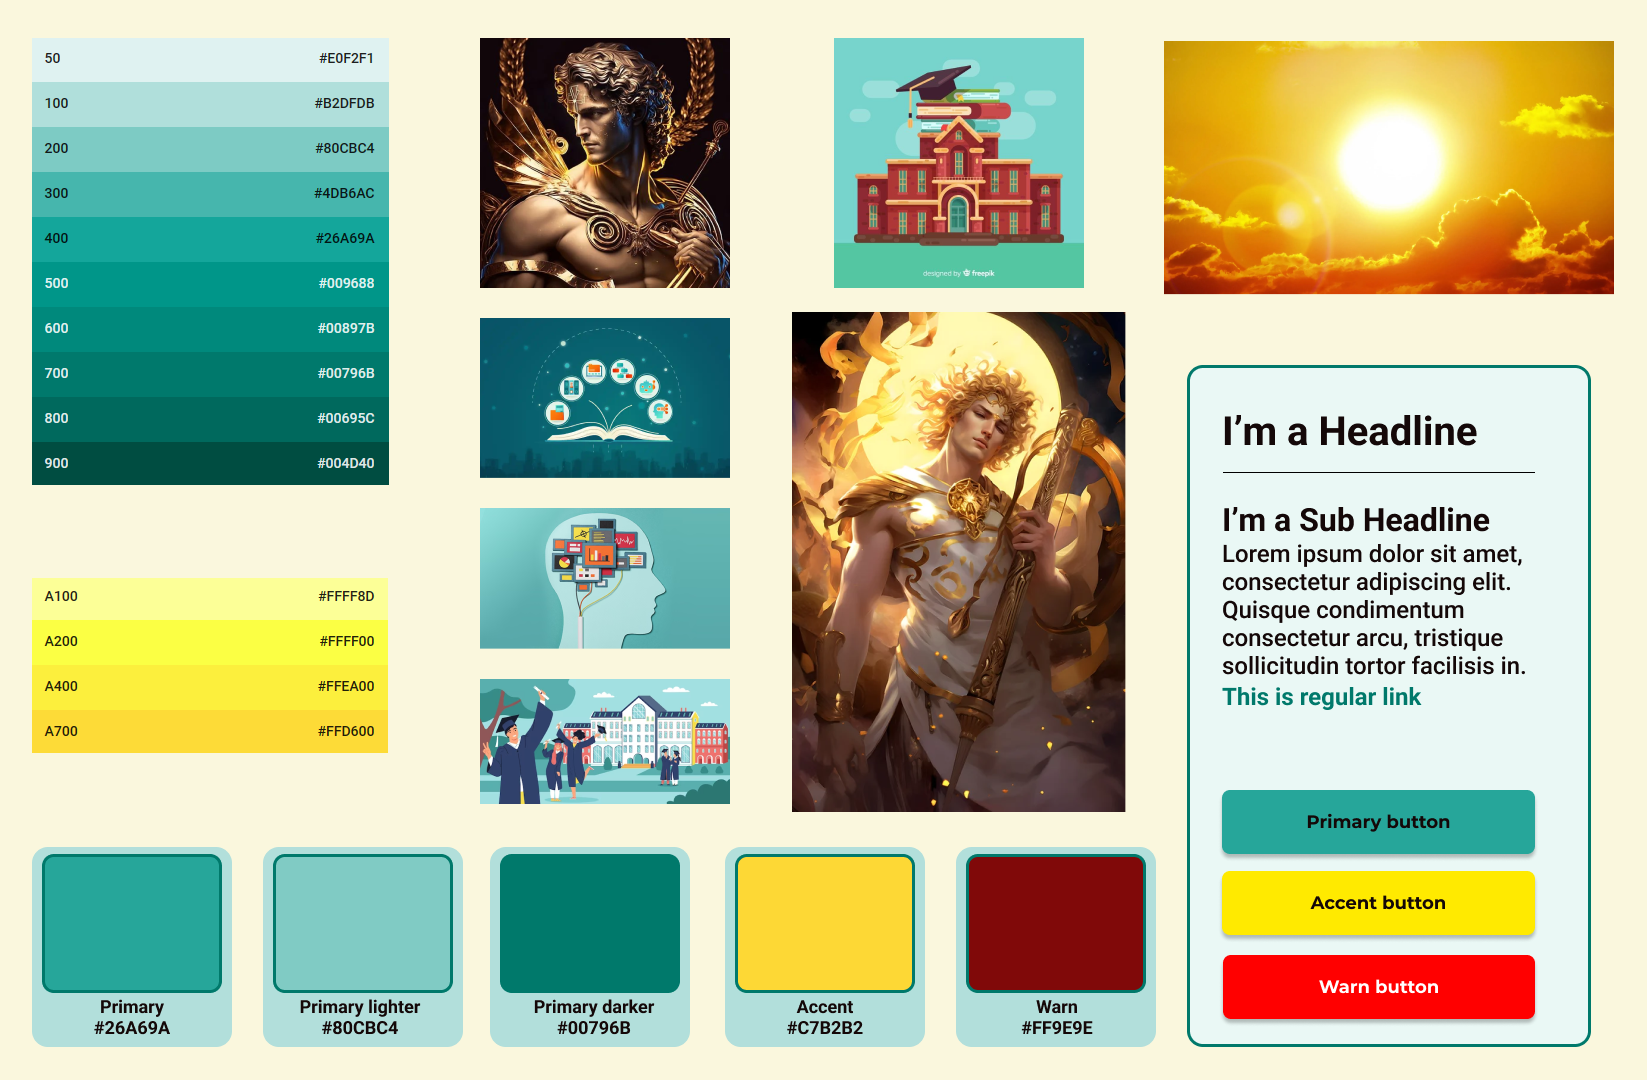
\includegraphics[width=1\linewidth]{moodboard1.png}
    \caption{Első hangulattábla}
    \label{fig:moodboard1}
\end{figure}

Az első hangulattábla (\ref{fig:moodboard1}. ábra) nem passzolt ezekhez az elképzeléseimhez, és a túl változatos színvilága nem érte el ezt az otthonosabb felhasználói élményt, ami az elsődleges célom volt. A második hangulattábla (\ref{fig:moodboard2}. ábra) véleményem szerint már sokkal jobbat teljesítette ezt az elvárásomat.

\begin{figure}
    \centering
    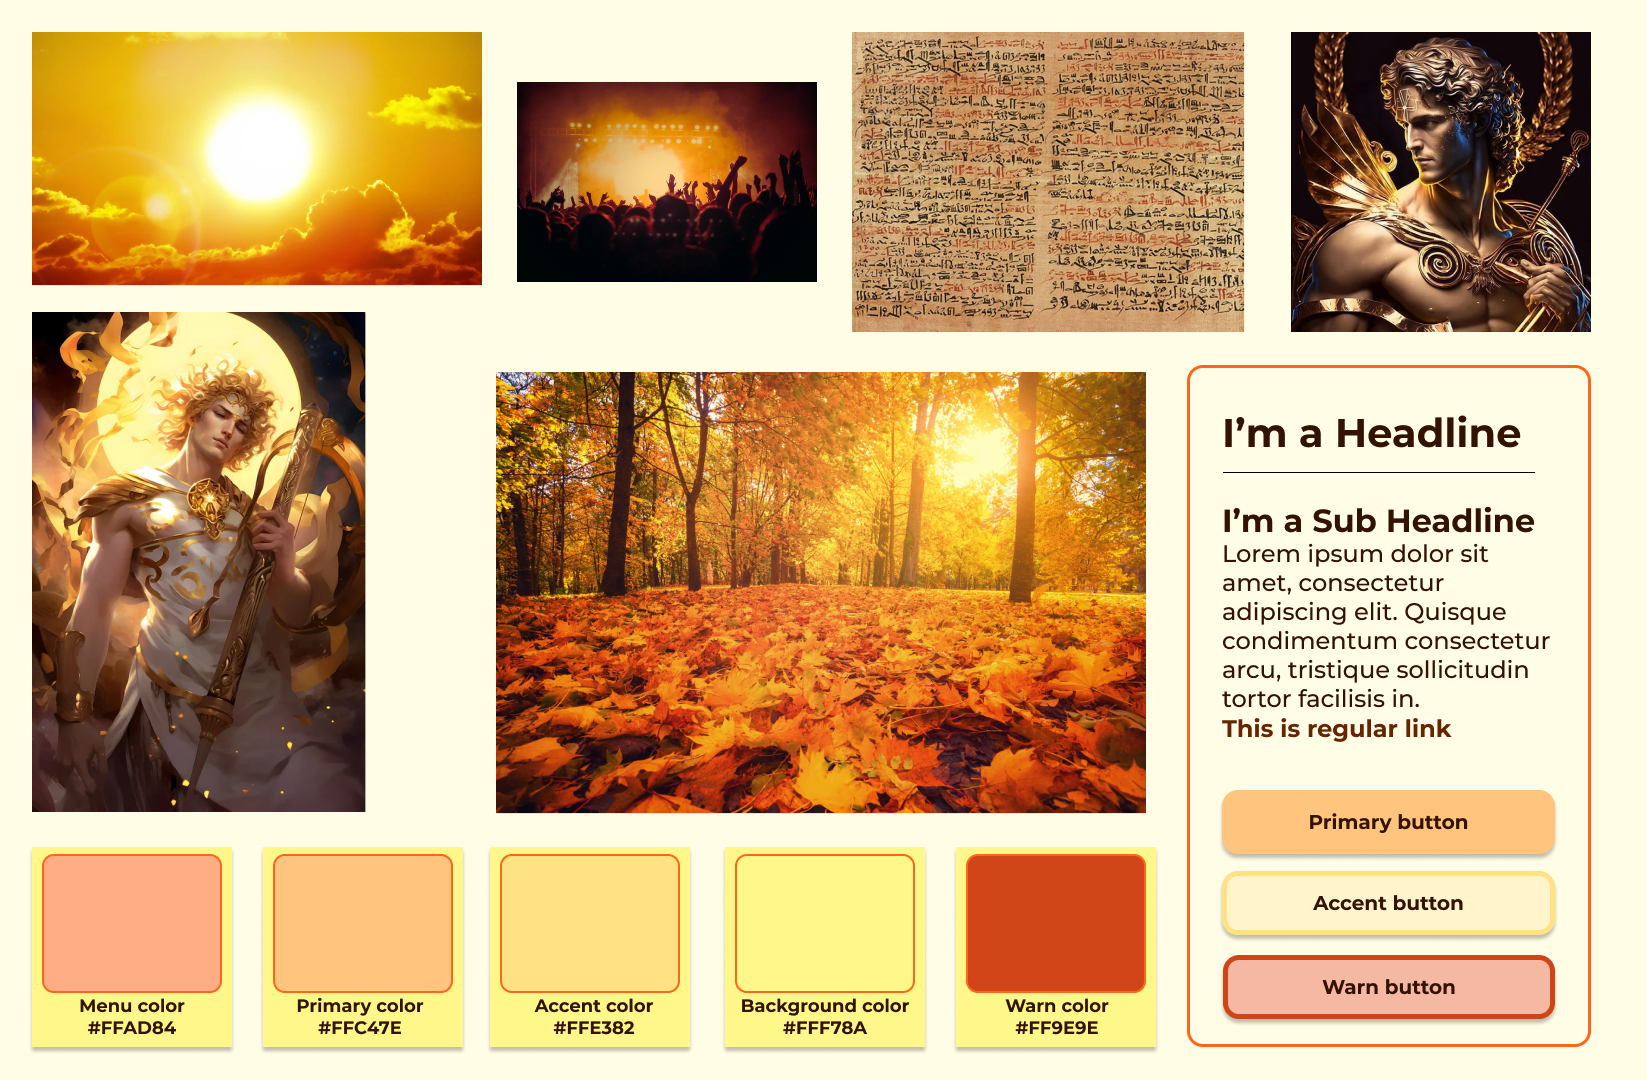
\includegraphics[width=1\linewidth]{moodboard2.png}
    \caption{Második hangulattábla}
    \label{fig:moodboard2}
\end{figure}

\chapter{Az alkalmazás működése}

\section{Használt technológiák}

Az alkalmazást Angularban \cite{angular} írtam, ami egy TypeScript keretrendszer, melyet az NPM (Node Package Manager) segítségével lehet buildelni és futtatni. 20.9.0-s Node.js verzióval dolgoztam, és 10.1.0-s NPM verzióval.

\subsection{Angular (17.0.0)}

Angular v17-et választottam a fő technológiának, amivel dolgozok, ugyanis munkahelyen széleskörű oktatást kaptam az Angular nagyméretű, összetett alkalmazások fejlesztéséhez való használatában, és mostanra már otthonosan mozgok benne. A v17-es a legújabb főverzió, továbbá számtalan olyan újítást hozott be a keretrendszerbe, amik további megoldásoknak nyitnak utat egy ilyen alkalmazás fejlesztésekor.

Fontos megemlíteni az Angular Material csomagot is, melyet a különböző komponensek (card, form field, tabs) miatt használtam, hogy egy letisztult, egységes kinézetet kölcsönözzenek a felhasználói felületnek.

\subsection{AngularFire (17.0.1)}

Az AngularFire a Firebase Angular-hoz készített csomagja. Az alkalmazás Firestore-t használ adatbázisként, amely bár nem képes sok backend-es funkciót ellátni, egy kezdetleges adatbázist képes szolgáltatni, mely megteremti a megfelelő körülményeket egy jól kigondolt frontend felépítéséhez.

\subsection{Transloco (6.0.4)}

A Transloco csomag az i18n (internationalization) irányelv többnyelvűsítésért felelős egyik csomagja. Lehetővé teszi, hogy futási időben változzon meg az alkalmazás nyelve, ezt a nyelvi forrásként szolgáltatott JSON fájlokba írt fordítások segítségével teszi meg. Mindenképpen szerettem volna többnyelvűre készíteni az alkalmazást, mert lehetővé szerettem volna tenni külföldi hallgatók általi használatát.

\subsection{NgRx (17.1.1)}

Az NgRx \cite{ngrx-store} egy állapotkezelő (state management) csomag, mely az RxJS reaktív adatfolyamjaira épülve egy összetett, skálázható módon oldja meg az adatok tárolását későbbi gyors betöltés céljából, valamint az oldalak állapotának megőrzését.

\subsection{jasmine (5.1.0)}

A jasmine csomag segítségével írtam egységteszteket az alkalmazás különböző részeihez. Felhasználtam továbbá a jasmine-marbles csomagot is a reaktív adatfolyamok teszteléséhez.

\subsection{További jelentős csomagok}

\begin{itemize}
    \item \textbf{lodash} (4.17.21): hasznos segédfüggvényeket tartalmazó csomag
    \item \textbf{NgxSpinner} (16.0.2): segédcsomag a töltőképernyőanimációkhoz
    \item \textbf{Angular Color Picker} (16.0.0): segédcsomag, mely egy színválasztó beviteli mező komponenst tartalmaz
    \item \textbf{read-excel-file} (5.8.1): segédcsomag a feltöltött Excel fájlok feldolgozásához
\end{itemize}

Az összes felhasznált NPM csomag a mellékletek \ref{fig:dependencies}. ábráján tekinthető meg.

\section{Modulok}

A fő funkciók alapján 4 modulra osztottam fel az alkalmazást, melyekhez tartozó adatokat egyértelműen el lehet különíteni. Ezek a következők:
\begin{itemize}
    \item tanulmányi átlagok,
    \item mintatantervbeli haladás,
    \item órarendtervező,
    \item admin oldal.
\end{itemize}
Ezeken kívül sok adat, komponens és service található az alkalmazásban, melyeket mindegyik, vagy legalább több modul is használja.

Ezek a modulok különálló oldalak, így köztük közvetlen kommunikáció nincs.

\subsection{Store}

A modulok közötti közvetett kommunikációért az NgRx csomag Store-ja felel, mely egy virtuális tárként működik az alkalmazásban. A Store-ba úgynevezett feature-öket lehet beregisztrálni, melyek az alkalmazás egyes moduljaival jönnek létre, ha a felhasználó az Angular Router segítségével az adott oldalra navigál, és betölti a modult.

\section{Adatmodell}

Az alkalmazás adatát nem osztályokon keresztül tároltam el, hanem TypeScript interfészekben, melyek sokkal rugalmasabb kezelhetőséget biztosítanak, és az adatbázissal való kommunikáció során sincs szükség különösebb átalakításokra, hiszen ezek gyakorlatilag egyszerű JavaScript objektumok (POJO).

Az adatbázisban tárolt objektumoknak string típusú az id mezője, mert a Firestore alapértelmezetten szöveges azonosítókat generál az eltárolt dokumentumoknak (rekordoknak), és én ezt a módszert használtam az objektumok azonosítására.

\subsection{Órarend}

Az órarend adata, mely \az{\ref{fig:data_model_timetable}.} ábrán látható, teljesen független az alkalmazás többi részétől, csak az órarendtervező oldalon került felhasználásra.

\begin{figure}[h]
    \centering
    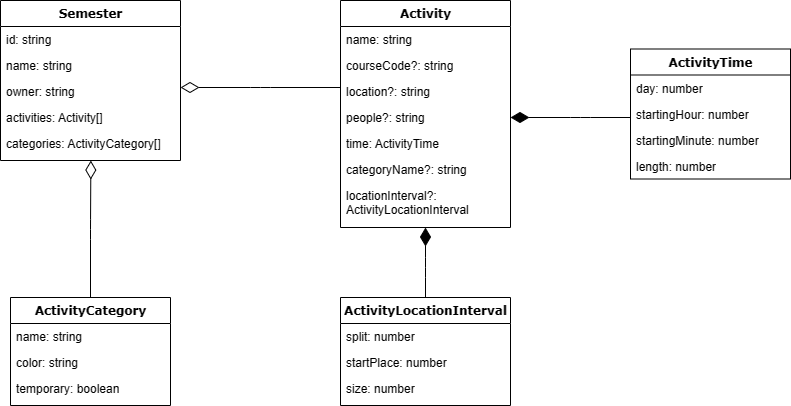
\includegraphics[width=1\linewidth]{órarendtervező_adatmodell.png}
    \caption{Az órarendtervező modul adatmodellje}
    \label{fig:data_model_timetable}
\end{figure}

A Firebase lehetővé teszi az egymásba ágyazott objektumok használatát, így egyetlen félévet is el lehet tárolni egy adatrekordban. Az ábrán látható objektumok fizikailag is tartalmazzák a megfelelő, hozzájuk tartozó objektumokat, az egyetlen külső kulcs kapcsolat az Activity interfész \textit{categoryName} adattagja, mely az ActivityCategory interfész \textit{name} adattagjára hivatkozik.

Az ActivityLocationInterval az egyetlen adat, mely nem az adatbázisban kerül az objektumokra. Ebben az interfészben tárolt adat határozza meg az órarendi tevékenységek megjelenését, mely az után számolódik ki, hogy betöltődtek az adatok az adatbázisból.

\subsection{Egyetemek}

Az egyetemek adatmodelljét (\ref{fig:data_model_universities}. ábra) több helyen is használtam (tanulmányi átlagok, mintatantervbeli haladás, admin oldal), habár módosítani csak az admin oldalon lehet. Azonban a felhasználói beállítások oldalon kiválaszthatja a felhasználó, hogy melyik egyetem melyik szakjára jár, valamint a tanulmányi átlagok és mintatantervbeli haladás oldalon lenyíló listából választhatja ki egy újonnan teljesített tárgyat, ezek adatai az egyetemek adataiból kerülnek ki. Továbbá a mintatantervbeli haladással kapcsolatos tárgycsoporti követelmények is ebben az adathalmazban vannak eltárolva.

\begin{figure}[h]
    \centering
    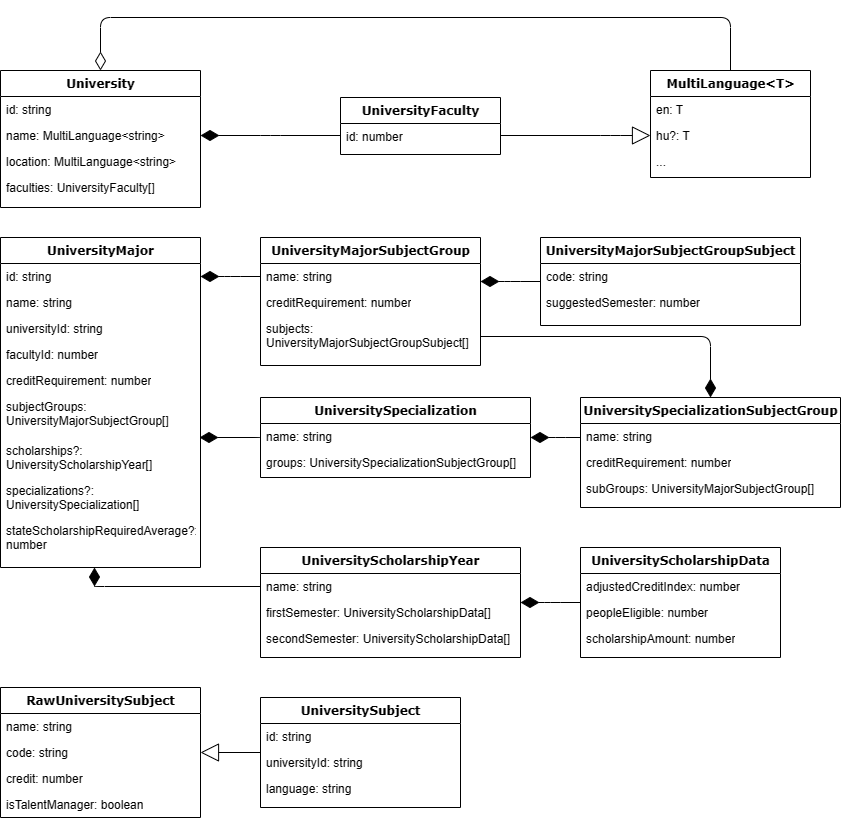
\includegraphics[width=1\linewidth]{egyetemek_adatmodell.png}
    \caption{Az egyetemi adatok modellje}
    \label{fig:data_model_universities}
\end{figure}

A MultiLanguage egy általánosan használt interfészem, melynek minden, az alkalmazásban elérhető nyelvre van egy mezője. Olyan objektumok (általában szövegek) lefordítására használom, melyek nem statikusak, ezért nem tudom a Transloco csomag segítségével lefordítani, hanem például adatbázisból érkeznek.

A RawUniversitySubject egy csak importáláshoz használt interfész, melyben azelőtt vannak az adatok, hogy hozzá lennének rendelve az aktuálisan kiválasztott egyetemhez, és az admin felhasználó megadná a nyelvüket. Ezt a segédinterfészt azért vezettem be, hogy addig is tudjam tárolni az adatokat egy egyszerűbb objektumban, amíg az importálási folyamat a végéhez nem érkezik.

\subsection{Teljesítések}

Az alkalmazás adatainak harmadik kategóriája a teljesítések, melyeket a tanulmányi átlagok és a mintatantervbeli haladás oldalon használja az alkalmazás. Egyaránt tárolja azt, hogy milyen tárgyakat teljesített a felhasználó, és azt is, hogy milyen érdemjeggyel végezte el őket. Az adatmodell \az{\ref{fig:data_model_completions}.} ábrán látható.

\begin{figure}[h]
    \centering
    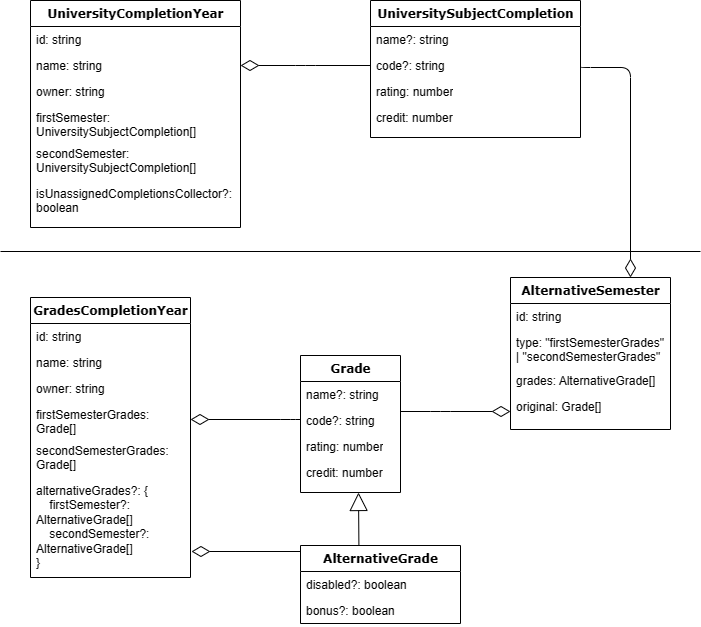
\includegraphics[width=1\linewidth]{teljesítések_adatmodell.png}
    \caption{A teljesítések adatmodellje}
    \label{fig:data_model_completions}
\end{figure}

A nagy hasonlóságot a UniversityCompletionYear és a GradesCompletionYear között az okozza, hogy míg az elválasztó feletti interfészeket a mintatantervbeli haladás oldalon használom, és ilyen formában vannak eltárolva a Store-ban a teljesítések, addig az elválasztó alatti interfészeket kizárólag a tanulmányi átlagok oldalon használom. Mindenképpen külön interfészt szerettem volna rá bevezetni, hogy jól el legyen különítve a két modul, még ha ugyanazt az adatot is használják, valamint ha a későbbiekben olyan adatok is kerülnek az alkalmazásba, amik csak az egyik modulban lesznek használva (például jelenleg az alternatív jegyek a tanulmányi átlagok oldalon), akkor a másik modul egyáltalán ne is jusson azokhoz az adatokhoz, adattagokhoz.

\section{A rendszer magasszintű folyamatai, működése}

Az alkalmazás nagy mennyiségű, összetett adattal dolgozik, és egy adatot sokszor az alkalmazás különböző részein is fel kell használni. Az így felmerülő adatfolyamok kezelésére választottam az NgRx csomagot, mely jól együtt tud működni a felhasználóval és az adatbázissal, mindezt az RxJS reaktív eszközeivel.

\subsection{Szekvencia diagram}

\Az{\ref{fig:SequenceDiagram}.} ábrán mutatom be egy szekvencia diagram segítségével az alkalmazásban előforduló, felhasználói interakciók nyomán kiváltott eseményeket. Az összes adatáramlást ennek a sémának a követésével igyekeztem implementálni, ezáltal egy egységes, könnyen átlátható felépítést adva az alkalmazás egyik központi részének.

\begin{figure}
    \centering
    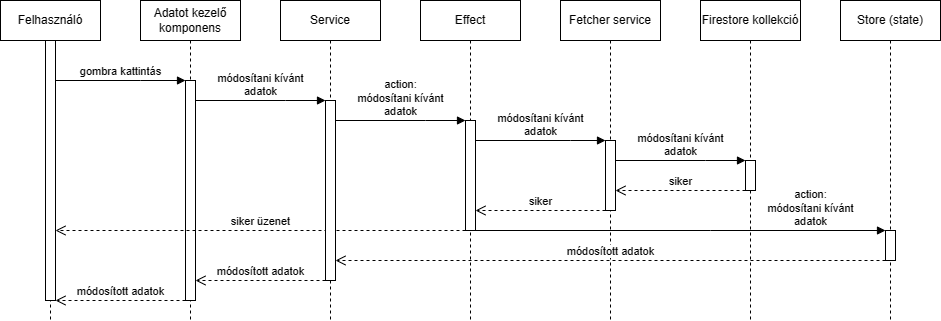
\includegraphics[width=1\linewidth]{szekvencia_diagram.png}
    \caption{Szekvencia diagram az alkalmazás általános adatáramlásainak}
    \label{fig:SequenceDiagram}
\end{figure}

A felhasználót külön vettem a komponenstől, ami a view megtestesítője, és az adatok felületes kezelője. Onnan az adat egy külső service-be jut, ami egy Angular építőelem, és a legtipikusabb feladata az adatközvetítés, és más service-ekkel való kommunikáció. Ez a service egy action-be csomagolja a módosítandó adatokat, amiket egy effect kezel, ami egy központi, aszinkron felület, ahol az alkalmazás különböző részeiből jövő action-ökre lehet reagálni. Itt először egy fetcher service-be küldi az adatokat (így neveztem egységesen a Firestore backend-del kommunikáló service-eket), majd onnan a Firestore-ba, ami kollekciókban tárolja az adatokat. Amikor jelez, hogy sikeres volt az adattárolás, az effect reagál rá, és egy újabb action segítségével elküldi az adatokat a Store-ba, ami az NgRx memóriában lévő tárolója.

A Store-ban történt változásokra reagál a service, és rajta keresztül a komponens is, ezáltal eljutnak a módosított adatok a felhasználóhoz. Fontos megemlíteni, hogy az effect a Store módosításával egyidőben küld egy üzenetet a felhasználónak, hogy sikeresen elvégezte a kívánt műveletet. Ez az üzenet egyidőben fog megérkezni a felhasználóhoz a módosított adatokkal, mert utána már nem történik adatbázis-kommunikáció, csak a memóriában tárolt adatok fognak mozogni az alkalmazásban, szinkron módon.

\subsection{Adatfolyam}

Az alkalmazás adatfolyamait az NgRx Store építőelemeivel a legegyszerűbb bemutatni, mert maga a Store felépítése a hagyományos adatfolyam diagramok építőelemeire hajaz. Ezeket az építőelemeket a szekvencia-diagram szereplőinek elnevezésekor is már használtam:
\begin{itemize}
    \item \textbf{state}: ezek digitális tárak, melyek az alkalmazás adatait tárolják a memóriában. A core state az alkalmazás elindulásakor jön létre, míg a feature state-ek csak akkor töltődnek be, ha az adott feature-höz tartozó modul létrejön.
    \item \textbf{action}: ezek felelősek az alkalmazás egyes részei közötti kommunikációért, valamint a state-ek frissítéséért és különböző mellékhatások elindításáért. Az adatfolyam diagramon egyes kapcsolatoknak felelnek meg.
    \item \textbf{effect}: ezek felelősek a mellékhatások közvetlen kezeléséért. Reaktív módon reagálnak az action-ökre, és azok alapján mellékhatásokat indítanak el. Az effect-ek felelősek külső API-k hívásáért is, ahonnan, ha megkapják a választ, újabb action-ök kilövésével tudják továbbítani a kapott adatokat. Az effect-ek tulajdonképpen egy keretet biztosítanak az adatfolyam diagram néhány, összetartozó folyamata körül.
    \item \textbf{reducer}: ezek frissítik a state-eket a megadott action-ök érkezésekor, a bennük szállított adatok alapján.
    \item \textbf{selector}: ezek segítségével reaktívan le lehet kérni a state-ekben tárolt adatokat, lehetővé téve, hogy az alkalmazás dinamikusan reagáljon minden adatváltozásra.
\end{itemize}

\Az{\ref{fig:data_flow_diagram}.} ábrán látható adatfolyam diagramon néhány részletet máshogy jelöltem, mint hagyományosan szokás, hogy ezáltal több részletet tüntethessek fel az ábrán. Mivel minden adattár digitális, ezért nem D betűvel neveztem el őket, hanem F vagy S betűvel, az alapján, hogy egy Firestore kollekcióról van szó, vagy pedig az NgRx egy State-jéről, amit éppen adattárként használunk. Ezenkívül a folyamatok köré egy keretet raktam, mely jelöli a folyamat lebonyolításának kontextusaként szolgáló NgRx effect-et. Továbbá a megfelelő kapcsolatok felett pluszban feltüntettem az alkalmazásban használt action nevét, mely az adott kapcsolatnak felel meg.

\begin{figure}
    \centering
    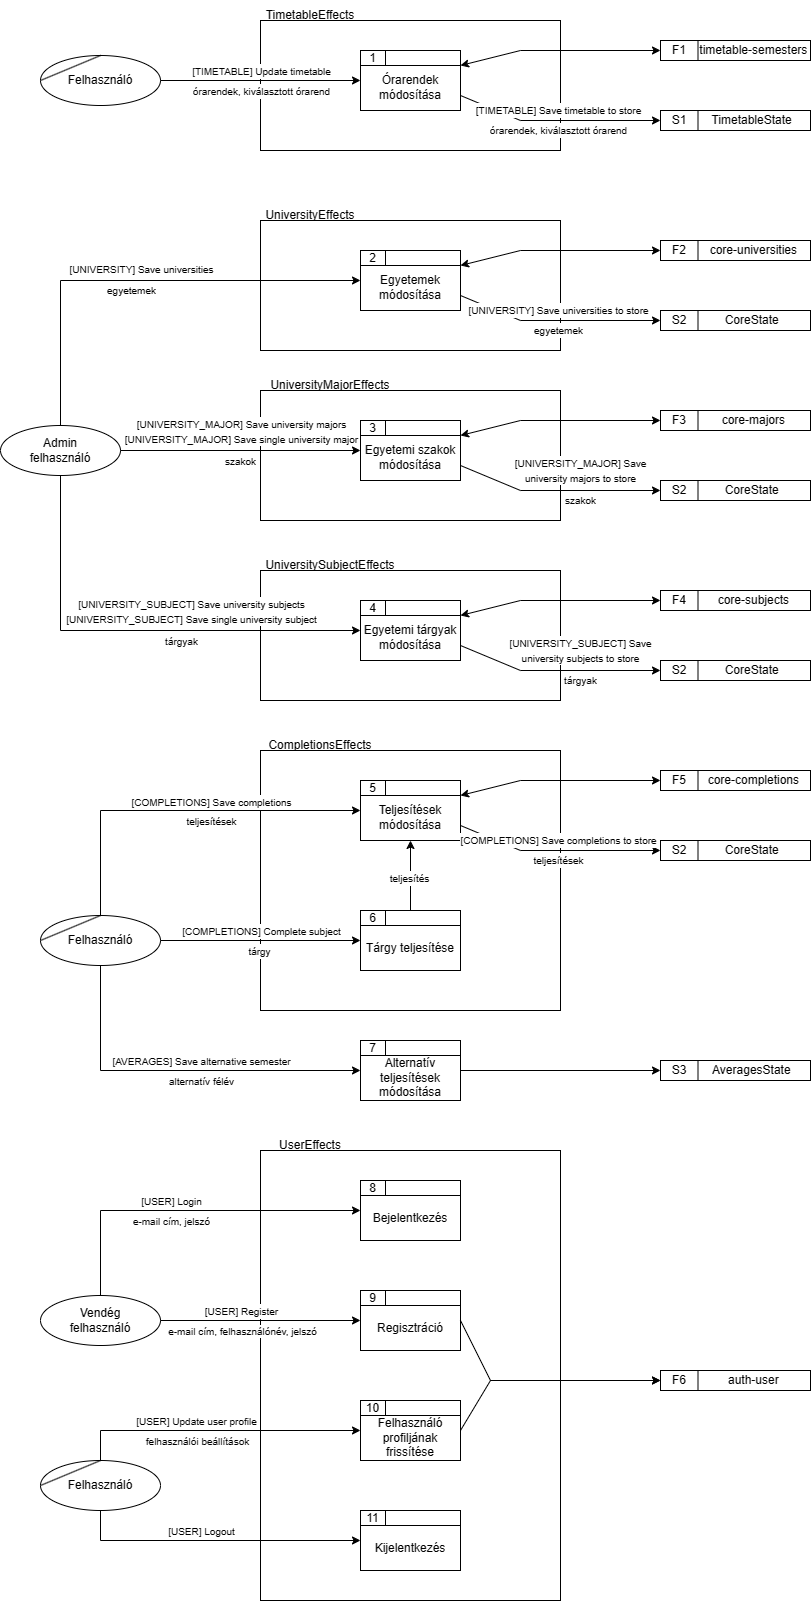
\includegraphics[width=0.7\linewidth]{adatfolyam_diagram.png}
    \caption{Adatfolyam diagram}
    \label{fig:data_flow_diagram}
\end{figure}

Az adatok frissítésének az általános folyama a következő: a felhasználó interakció által egy action lövődik ki, melyet az adott effect dolgoz fel. Először frissíti a Firestore adatbázist, majd a memóriában lévő NgRx Store-t is.

\section{Fontosabb kódrészletek}

\subsection{Az adat útja}

Egy konkrét példán keresztül szeretném bemutatni, hogy hogyan jut el az adat a felhasználótól az adatbázisig, majd vissza a felhasználóhoz, már megjelenítéskor. A mintatantervbeli haladás oldalon a teljesítések elmentése folyamatot mutatom be, melyet a felhasználó egy adatszerkesztő dialógusban tud elindítani a "Mentés és bezárás" gomb megnyomásával.

A HTML template-en kerül interakcióba a felhasználó az alkalmazással, itt kattint rá a gombra, melynek a \verb|click| \verb|EventEmitter|-e meghívódik, ezáltal a dialógus komponens \verb|save| metódusa is. A gombhoz egy saját \verb|apo-button| komponenst használtam, hogy könnyebben egységesíthessem az alkalmazásban mindenhol megjelenő gombok kinézetét és működését.

\pagebreak
\begin{samepage}
    \begin{verbatim}
<apo-button apoRole="save"
  (click)="save()">
  {{ "GENERAL_BUTTON_LABELS.SAVE_AND_CLOSE" | transloco }}
</apo-button>
    \end{verbatim}
\end{samepage}

Mentéskor a komponens először az RxJS eszköztárával lekéri az éppen bejelentkezett felhasználót a \verb|UserService| segítségével, majd egy utility osztály metódusával átalakítja a komponensben használt speciális alakú adatokat az adatbázisban is tárolt adatokká, a bejelentkezett felhasználó e-mail címét beleírva az adatokat tároló objektumokba. Amint ezzel végzett, bezárja a dialógust, visszaadva ezeket az adatokat a dialógust megnyitó metódusnak.

\begin{samepage}
    \begin{verbatim}
public save(): void {
  this.userService.user$.pipe(
    take(1),
    map(user => user!.email)
  ).subscribe(email => this.dialogRef.close(
    CompletionMapperUtils.mapSubjectCompletionsToCompletionYears(
      this.completions(), email
    )
  ));
}
    \end{verbatim}
\end{samepage}

(Megjegyzés: a kódrészletben a \verb|CompletionMapperUtils| metódusának a neve a forráskódban \textit{mapManagableSubjectCompletionsToCompletionYears}, itt azért rövidítettem le, hogy kiférjen a dokumentumban.)

A dialógust megnyitó metódus (\verb|open()|) eredményének (ami egy dialógus referencia) \verb|afterClosed| függvényhívása után érkeznek meg a dialógus által visszaadott adatok. Hogyha léteznek, tehát a felhasználó a mentés gomb segítségével zárta be a dialógust, akkor a \verb|CompletionsService| mentés metódusa hívódik meg a menteni kívánt adatokkal.

\pagebreak
\begin{samepage}
    \begin{verbatim}
public manageCompletions(): void {
  this.dialog.open(
    CompletionManagerDialogComponent, {
      data: {
        completions: this.userCompletions(),
         universitySubjects: this.universitySubjects()
      }
    }
  ).afterClosed().subscribe(updatedCompletions => {
    if (!updatedCompletions) {
      return;
    }
    this.completionsService.saveUniversityCompletions(
      updatedCompletions
    );
  });
}
    \end{verbatim}
\end{samepage}

Mentéskor először egy ellenőrzést végez a metódus, hogy ha a teljesített tárgyak között van olyan tárgy, amihez még nincs rendelve félév (ha a mintatantervbeli haladás oldalon a gyors mentés gombra kattintunk egy tantárgy mellett, akkor jöhet elő ez a helyzet), viszont valamelyik félévben is már fel van véve ez a tárgy (pl. a tanulmányi átlagok oldalon felvette a felhasználó), akkor, hogy ne legyen duplikálva, kitörli azt, amelyikhez nincs félév rendelve. Ez a felhasználói élmény céljából történik, hogy ne kelljen a felhasználónak kézzel kitörölnie a félévhez nem rendelt teljesítményt. (A teljes metódus a mellékletek között \az{\ref{fig:CompletionsService.saveUniversityCompletions}.} ábrán látható.)

A metódus alján hívódik meg az NgRx Store \verb|dispatch| metódusa, mellyel egy \textit{[COMPLETIONS] Save completions} típusú action-t lő ki a módosított, elmentendő teljesítésekkel.

\pagebreak
\begin{samepage}
    \begin{verbatim}
public saveUniversityCompletions(
  completions: UniversityCompletionYear[]
): void {
  completions = cloneDeep(completions);

  ... (szűrés)

  this.store.dispatch(
    completionsActions.saveCompletions({ completions })
  );
}
    \end{verbatim}
\end{samepage}

A \verb|CompletionsEffects| megfelelő adattagja, egy effect, fogadja az összes, az alkalmazásban kilőtt action-t. Először kiszűri a \textit{[COMPLETIONS] Save completions} típusúakat, majd megnyit egy töltőképernyőt, tájékoztatva a felhasználót az adatbázissal való, potenciálisan időigényes kommunikációról. Ezt követően a \verb|CompletionsFetcherService| (az a service, ami már a Firestore adatbázissal kommunikál) megfelelő metódusát meghívva elmenti az adatbázisba az új teljesítéseket, majd amint az visszajelez sikeres adatbázistranzakcióval, a választ átalakítja egy \textit{[COMPLETIONS] Save completions to store} típusú action-re, és bezárja a töltőképernyőt. Mivel az effect ezzel az action-nel tér vissza, ezért ennek is olyan hatása lesz, mint a Store \verb|dispatch| metódusának, egy action-t lő ki az effect.

Az Observable pipeline végén a hibák is le vannak kezelve, melyek az adatbázissal való kommunikáció közben léphetnek fel. Ekkor nem lő ki semmilyen action-t az effect, csak bezárja a töltőképernyőt, és egy kis üzenetet jelenít meg a képernyő alján, mely tájékoztatja a felhasználót a hibáról.

\pagebreak
\begin{samepage}
    \begin{verbatim}
public readonly saveCompletions$ = createEffect(() =>
  this.actions$.pipe(
    ofType(completionsActions.saveCompletions),
    tap(() => 
      this.loadingService.startLoading(
        completionsLoadingKey,
        LoadingType.SAVE
      )
    ),
    switchMap(({ completions }) =>
      this.completionsFetcherService.saveCompletions(completions).pipe(
        map(() => {
          this.loadingService.finishLoading(completionsLoadingKey);
          return completionsActions.saveCompletionsToStore(
            { completions }
          );
        })
    )),
    catchError(() => {
      this.loadingService.finishLoading(completionsLoadingKey);
      this.snackbarService.openError("ERROR.DATABASE.COMPLETIONS_SAVE");
      return [];
    })
  )
);
    \end{verbatim}
\end{samepage}

Ezt az action-t nem egy effect fogja kezelni, hanem egy reducer, ami a megadott függvény alapján megváltoztatja a Store-nak azt a state-jét, ami a teljesítések tárolásáért felel. Ebben az esetben egyszerűen felülírja a korábbi teljesítéseket az újakra.

\pagebreak
\begin{samepage}
    \begin{verbatim}
on(
  completionsActions.saveCompletionsToStore,
  (state, { completions }) => (
    { ...state, completions: completions }
  )
)
    \end{verbatim}
\end{samepage}

A \verb|CompletionsService|-ben egy Observable továbbítja az aktuális teljesítéseket, melyeket közvetlenül a Store-ból kér le egy selector segítségével. A state állapotának változásakor az új adatok automatikusan megérkeznek a selector-on keresztül, melyet a service először leellenőriz, hogy biztosan léteznek-e. (Az alkalmazás indulásakor még nem léteznek, ez azt a kezdeti betöltést kezeli le.) Ha nem, kilő egy action-t, ami le fogja kérni az adatbázisból a teljesítéseket. Hogyha viszont léteznek, akkor tovább folyik az adat. (A \verb|multicast| egy saját operátor, mely hot Observable-lé alakítja az adatfolyamot, a \verb|distinctUntilChanged| pedig a paraméterben adott metódus segítségével egyenlőséget vizsgál, és csak akkor küldi tovább az adatot, ha különbözik az előzőként érkezőtől, ezáltal szűrve a felesleges adatáramlásokat.)

\begin{samepage}
    \begin{verbatim}
this.universityCompletions$ = this.store.select(
  coreFeature.selectCompletions
).pipe(
  tap(completions => {
    if(!completions) {
      this.store.dispatch(completionsActions.loadCompletions());
    }
  }),
  filter(Boolean),
  multicast(),
  distinctUntilChanged(isEqual)
);
    \end{verbatim}
\end{samepage}

A mintatantervbeli haladás oldal komponense lekéri a \verb|CompletionsService|-ből a teljesítések adatfolyamát, melyet egy Signal-lé (egy reaktívan becsomagolt értékké) alakítja. Amíg nem érkezik adat az adatfolyamon (ez megint csak az alkalmazás indulásakor fordulhat elő), egy üres tömbnek tekinti a teljesítéseket.

A \verb|takeUntilDestroyed| operátor a memóriaszivárgások elkerülése végett része a pipeline-nak. Ez az operátor teszi lehetővé, hogy a komponens megszűnésekor (azaz az alkalmazás bezárásakor vagy más oldalra navigáláskor) leiratkozzon erről az Observable-ről. Az observer tervezési minta értelmében pedig ilyenkor, ha nincs más observer-e az adatfolyamnak, az megszűnik, ezáltal nem használ felesleges memóriát.

\begin{samepage}
    \begin{verbatim}
this.userCompletions = toSignal(
  this.completionsService.universityCompletions$.pipe(
    takeUntilDestroyed(),
    startWith([])
  )
) as Signal<UniversityCompletionYear[]>;
    \end{verbatim}
\end{samepage}

A komponens HTML template-jén pedig használva van a Signal értéke (szintaktikailag egy egyszerű függvényhívásnak néz ki), többek között a hiányzó kreditek kiszámításához, valamint a még teljesítetlen tárgyak szűréséhez. Ez a mellékletek között \az{\ref{fig:MajorCompletionComponentTemplate}.} ábrán látható.

Megjegyzem, hogy a legelső kódrészleten látható ennek a Signal-nek a használata, amikor a jelenlegi értékekkel megnyitásra kerül az adatszerkesztő dialógus.

Az alkalmazás egészében kisebb-nagyobb adatátalakító függvények hívásán kívül többnyire így néz ki az adatfolyam a felhasználó és az adatbázis, valamint a Store között.

\subsection{Regisztráció}

A regisztráció folyamatában az volt a kihívás, hogy szerettem volna lehetőséget nyújtani a felhasználónak, hogy ha előtte már vendégként használta az alkalmazást, akkor az ott felvitt adatokat (tanulmányi jegyek és órarendi órák) a kérésére az alkalmazás átvigye a frissen regisztrált fiókjába.

Ezt is, ahogy az alkalmazás összes adatmanipuláló eseményét, egy effect végzi, a \verb|UserEffects| osztályban. Az effect egy adattagként lesz beregisztrálva, mely az NgRx Store action-jeit olvassa. Kiszűri ezek közül a \textit{[USER] Register} típusúakat, amikkel foglalkozni akar az effect, majd megnyit egy töltőképernyőt. Ezt követően lefolytatja a Firebase Auth-tal való kommunikációt, amikor létrehozza a felhasználó fiókját, majd ezt követően elmenti az adatait Firestore-ba, melyeket a regisztráláskor megadott. Hiba esetén üzenetet mutat a sikertelen felhasználói adatmentésről a felhasználónak. Az eddigi folyamat \az{\ref{fig:UserEffectsRegister1}.} ábrán látható.

Ezután a függvény lekéri a vendégfelhasználó adatait, melyeket a böngészőben tárol, úgyhogy szinkron módon eléri, és leellenőrzi, hogy vannak-e mentett adatok. Ha nincsenek, kilő egy action-t, mely kiüríti a felhasználói adatokat a Store-ból, hogy ne a vendégadatok jelenjenek meg (amik potenciálisan mások is lehetnek, mint a jegyek és az órarendi órák), hanem az újonnan regisztrált felhasználó adatai. Ha vannak adatok, megállapítja, hogy a két, vendégeknek is elérhető oldal közül melyiken, majd a megfelelő szöveggel felnyit egy dialógust, ami megkérdezi a felhasználót, hogy szeretné-e megtartani a vendégadatait, vagy sem.

A felhasználó döntése alapján partícionáltam az Observable-t: ha szeretné megtartani, akkor egyből elmenti az adatait (mivel korábban megtörtént a bejelentkezés, így már a frissen regisztrált felhasználó számára), majd törli a vendégadatokat a böngészőből, eközben felmerülő hibák esetén pedig hibaüzenetet jelenít meg a felhasználónak. Ha nem szeretné megtartani az adatokat a felhasználó, egyszerűen egy action-nel törli az adatait Store-ból, ahogy akkor tette a program, amikor nincs a felhasználónak vendégadata. Ezt a két Observable-t egyesítem, mert a folyamat további része megegyezik, bármelyiket is választotta a felhasználó. Az ezekhez a részekhez kapcsolódó kódrészlet \az{\ref{fig:UserEffectsRegister2}.} ábrán látható.

Az utolsó része az effect-nek csak a töltőképernyő bezárásából, és hibakezelésből áll. Valamint kiszűrésre kerülnek azok az adatok, amik valójában nem tartalmaznak semmit, nem von maga után további akciókat, például amikor a felhasználó szeretné átvinni a vendégadatait (ekkor ugyanis nincs szükség a felhasználói adatok Store-ból való kiürítésére). Ez a mellékletek \ref{fig:UserEffectsRegister3}. ábráján tekinthető meg.

\chapter{Tesztelés}

Az alkalmazásban egységtesztelést \cite{angular-testing} valósítottam meg, mely a jasmine nevű csomaggal és a Karma nevű csomag segítségével történt meg. 160 különböző tesztesetet írtam az alkalmazásra, amik főleg a mögöttes logikát, számításokat és a bonyolultabb aszinkron folyamatokat tesztelik le.

Felhasználói tesztelés keretein belül továbbá leteszteltem az egyes funkciókat és azok együttműködését.

Néhány egységtesztre fogok példát mutatni.

\section{Az órarend pozícionálását végző utility osztály tesztelése}

Az órarend pozícionálását végző utility osztályt (\verb|TimetableSplitUtils|) könnyű volt tesztelni, mert bár egy bonyolult, több száz kódsoros algoritmus áll a hátterében, a különböző órarendi elemek egymáshoz viszonyított helyzetét könnyen el tudja képzelni az ember, így elég volt a végeredményre, a tevékenységek pozícionálás kiszámítása utáni helyzetére írni teszteket, nem pedig a részletes algoritmusra vagy belső segédfüggvényekre.

A teszteket először is egy külső \verb|describe| blokkba\footnote{Ez valójában nem egy blokk, hanem egy callback függvény, amit a tesztrendszer fog meghívni. Azért hivatkozok rá blokként, mert könnyebb róla úgy beszélni, és elképzelni is, mint egy blokk, aminek adott funkciója van.} szokás elhelyezni, ami egy kontextust ad, hogy éppen melyik osztály kerül tesztelésre. Ide kerülnek a teszteléssel kapcsolatos azon előkészületek, amik az egész osztály tesztelésére vonatkoznak. Itt egy utility osztályt tesztelek, így nincs szükség ilyen előkészületekre.

\pagebreak
\begin{samepage}
    \begin{verbatim}
describe('TimetableSplitUtils', () => { ... });
    \end{verbatim}
\end{samepage}

Eggyel beljebbre is kerül egy \verb|describe| blokk, amennyiben egy osztály metódusa lesz letesztelve, akkor a metódusnak is érdemes kontextust adni, amin belülre több teszteset is kerülhet. Ide az adott metódussal vagy adattaggal kapcsolatos tesztelőkészítéseket kell írni, például egy tesztadatot.

\begin{samepage}
    \begin{verbatim}
describe('splitTimetable', () => {
  const defaultLocationInterval: ActivityLocationInterval = {
    split: 1,
    startPlace: 0,
    size: 1
  };

  ...
});
    \end{verbatim}
\end{samepage}

A teszteseteket egy \verb|it| blokkba kell helyezni, mely megad egy funkcionalitást, amit annak a függvénynek el kell látnia, és amit a teszteset ellenőriz. A \verb|TimetableSplitUtils| osztály első tesztesete az egymással nem ütköző tevékenységek pozícionálását teszteli le, hogy valóban mindegyik teljes szélességgel helyezkedik-e el az órarenden.

\begin{samepage}
    \begin{verbatim}
it(
  "should leave activities with no intersecting duration",
  () => { ... }
);
    \end{verbatim}
\end{samepage}

Először egy segédfüggvénnyel létrehoztam a megfelelő órarendet, majd meghívtam a tesztelendő osztály tesztelendő metódusát ezekkel az adatokkal.

\pagebreak
\begin{samepage}
    \begin{verbatim}
const semester = createSemester(
  { day: 1, startingHour: 8, startingMinute: 0, length: 120 },
  { day: 1, startingHour: 10, startingMinute: 0, length: 60 },
  { day: 2, startingHour: 8, startingMinute: 0, length: 60 }
);

const splitSemester = TimetableSplitUtils.splitTimetable(semester);
    \end{verbatim}
\end{samepage}

A teszteket a jasmine csomag \verb|expect| metódusával lehet elvégezni, mely ebben az esetben objektumok egyenlőségét vizsgálja.

\begin{samepage}
    \begin{verbatim}
expect(splitSemester.activities[0].locationInterval).toEqual(
  defaultLocationInterval
);
expect(splitSemester.activities[1].locationInterval).toEqual(
  defaultLocationIntervalű
);
expect(splitSemester.activities[2].locationInterval).toEqual(
  defaultLocationInterval
);
    \end{verbatim}
\end{samepage}

Azért nem az egész \verb|splitSemester.activities| tömb egyenlőségét vizsgáltam a példa tesztadatok függvényében a kívánt eredménnyel, mert a tevékenységek egyéb adattagjai (neve, helyszíne, stb.) egyáltalán nem relevánsak a tesztek szempontjából. Amennyiben ezt is tesztelném, a kódban olyan változtatások rontanák el a teszteseteket, melyek nem is számítanának hibának a program futása szempontjából.

Egy másik tesztesetben azt szeretném kiemelni, hogy a jasmine rugalmasságot enged meg a tesztekben, például nem feltétlenül kell két objektum minden adattagjának egyeznie, megengedhetjük, hogy valamelyik adattag értéke bármi (de egy adott típusból, például egy szám) legyen. A mellékelt \ref{fig:TimetableSplitUtilsTestJasmineAny}. ábrán látható kódrészletben nem a pozícionált tevékenység minden adattagját ellenőriztem, csak hogy a teljes szélesség harmada a szétosztási alapegység (split), és összesen kettő ilyen alapegységet foglal el a tevékenység (size). Azt, hogy melyik helyen kezdődik (startPlace) felesleges ellenőriznem, mert irreleváns a működés szempontjából, hogy az első kettő vagy az utolsó kettő helyet foglalja el.

\section{A regisztráció tesztelése}

Az effect-ek tesztelése egy összetettebb folyamat, hiszen aszinkron adatfolyamokat kell ellenőrizni, hagyományos értékellenőrző \verb|expect|-ekkel nem lehet ezt megtenni. A jasmine csomag is többféle megoldást mutat erre, de talán a legletisztultabb módszer, amit én is alkalmaztam, az az RxJS marble testing \cite{rxjs-marbles}, melyet a jasmine egy külön csomaggal is támogat.

Angular-ban a legtöbb osztályt nem olyan egyszerű tesztelni az Angular dependecy injection rendszere miatt. Biztosítani kell ezeknek az osztályoknak a függéseiket, de hogy a megfelelő tesztelési környezetben fussanak, függetlenül az alkalmazás többi részének működésétől, ezért mock (utánzat) függéseket szokás adni az osztályoknak tesztelés során.

A tesztek előkészítése a későbbiekben felhasználásra kerülő objektumok deklarálásával kezdődik a külső \verb|describe| blokkon belül. A tesztelni kívánt effect valós objektum, a többi viszont csak a jasmine által biztosított spy objektum.

\begin{samepage}
    \begin{verbatim}
let effects: UserEffects;
let actions$: TestColdObservable;
let authService: jasmine.SpyObj<AuthService>;
let userFetcherService: jasmine.SpyObj<UserFetcherService>;
    \end{verbatim}
\end{samepage}

Az alapvető értékek megadása után a függéseket elkészítő factory függvényeket definiáltam, melyek egy jasmine spy objektumot készítenek el. Ezekben az objektumokban a használt metódusoknak felül van írva a visszatérési értékük, ezáltal elérhetjük, hogy a hívó fél le tudja futtatni, még ha a függvény valójában nem is létezik, csak ez a spy függvény ad vissza neki egy előre megadott értéket.

\begin{samepage}
    \begin{verbatim}
function authServiceFactory() {
  const service = jasmine.createSpyObj(
    'AuthService',
    ['signInUser', 'registerUser', 'signOutUser']
  );
  service.signInUser.and.returnValue(of(undefined));
  service.registerUser.and.returnValue(of(undefined));
  service.signOutUser.and.returnValue(of(undefined));
  return service;
}
    \end{verbatim}
\end{samepage}

Ezt követően konfigurálni kell a tesztelési környezetet biztosító modult. Ezt minden teszteset előtt újra létre kell hozni, hogy egymástól teljesen függetlenül lehessen a teszteket futtatni, ezért van egy \verb|beforeEach| blokkban.

A \verb|TestBed| az Angular tesztelésre tervezett segédje, melynek a \verb|configureTestModule| függvényével lehet létrehozni a tesztmodult. Itt kell megadni a függőségeket, vagy hogy miket használjon helyettük. Minden függőséghez provide-oltam a megfelelő factory függvényt, ami létre fogja hozni a spy objektumot, vagy pedig a konkrét spy objektumot, amikor nem kellett átállítani a létrehozandó spy metódusainak visszatérési értékét. Ez olyan metódusoknál fordulhat elő, amiknek csak mellékhatása van. Az elején látszik, hogy az NgRx tesztelési segédfüggvényét, a \verb|provideMockActions|-t használtam, aminek megadtam egy teszt Observable-t. Ez fogja szimulálni a kilőtt action-ök adatfolyamát a tesztelés során.

\begin{samepage}
    \begin{verbatim}
beforeEach(() => {
  TestBed.configureTestingModule({
    providers: [
      UserEffects,
      provideMockActions(() => actions$),
      {
        provide: AuthService,
        useFactory: authServiceFactory
      },
      {
        provide: SnackBarService,
        useValue: jasmine.createSpyObj(
          'SnackBarService',
          ['open', 'openError']
        )
      },
      ...
    ]
  });
    \end{verbatim}
\end{samepage}

Végül az elején deklarált változóknak adtam értékül a függőségeket, melyeket ellenőrizni akarok a későbbiekben. Ezeket jasmine-es spy objektumokká kasztoltam át.

\pagebreak
\begin{samepage}
    \begin{verbatim}
effects = TestBed.inject(UserEffects);
authService = TestBed.inject(AuthService) as jasmine.SpyObj<AuthService>;
snackbar = TestBed.inject(SnackBarService)
  as jasmine.SpyObj<SnackBarService>;
    \end{verbatim}
\end{samepage}

A regisztráció effect-jének a tesztjéhez nem elég például egy függvényt meghívni, mert egy action-t kell küldeni, hogy aktiválódjon az effect. Erre például egy megoldás, hogy a \verb|cold| függvénnyel létrehoztam egy teszt Observable-t, melynek egy marble diagram-mal adtam meg az adatfolyamát (egyetlen "a" értéket küld, melynek a tartalma a második paraméterben van megadva, egy regisztráció action a megfelelő tesztadatokkal). Ezt az Observable-t fogja a teszteset az action-ök folyamának használni, ami alapján le tud futni az effect.

Feliratkoztam az adatfolyamra, mert ekkor fog csak lefutni, viszont ez után még meg kell hívni a jasmine \verb|TestScheduler| \verb|flush| metódusát, hogy az aszinkron események lefussanak. (Valójában nem futnak le aszinkron események, csak a jasmine marbles képes szimulálni a teszt Observable-ök segítségével.) Ezek után le lehet ellenőrizni, szintén a jasmine spy-ok eszköztárával, hogy az adott service metódusa meghívódott-e a megfelelő paraméterekkel, azaz ez esetben beregisztrálta-e a felhasználót az effect.

A következő tesztesetben azt ellenőriztem, hogy az effect a megfelelő action-t emittálta-e, azaz egy aszinkron adatfolyam értékét kellett tesztelni. Ehhez a jasmine \verb|toBeObservable| metódusát használtam, ami feliratkozik az adott adatfolyamra (most az effect register\$ Observable-jére), majd leellenőrzi, hogy egyezik-e a megadott jasmine marble Observable-lel.

Mind a két teszt a mellékletek \ref{fig:UserEffectsSpecRegister}. ábráján látható.

\chapter{Tapasztalatok, továbbfejlesztési lehetőségek}

\section{Tapasztalatok}

Az alkalmazás elkészítése közben rengeteg tapasztalatot szereztem egy komplex, sok adattal dolgozó alkalmazás felépítésével kapcsolatban. A tervezés fontosságával is megismerkedtem, mert eddig még nem készítettem ilyen méretű alkalmazást előzetes tervekkel, habár az agilis szemléletmódból is merítettem, és amikor úgy éreztem, hogy a gyakorlat mást diktál, mint a tervek, akkor nem haboztam változtatni rajtuk.

Sokat tanultam ezen kívül az Angular v17 verziójáról is, és annak újdonságairól, mert ez volt az első projektem ebben az Angular verzióban. A Signal-ök \cite{angular-signals} egy vadonatúj irányzatát hozzák be az Angular-ba a reaktív programozásnak, és sok időt tölthettem ennek a megismerésével, és a vele való kísérletezéssel.

Mindezen kívül ebben az alkalmazásban sok külső csomagot használtam, ami egy nagyon hasznos tapasztalatnak bizonyult. Nem sokszor tapasztalhattam meg eddig azt az érdekes folyamatot, ami ott kezdődik, hogy van egy megoldandó problémám (az Apollo esetében például az Excel fájlokból való olvasás), és el kell döntenem, hogy saját magam implementáljam le, vagy pedig keressek egy csomagot, ami elvégezheti ezt a munkát számomra. Amennyiben pedig találok ilyen csomagot, az mennyire elégíti ki az igényeimet, milyen kompromisszumokat kell kötnöm, és milyen személyre szabási lehetőségeim vannak.

\section{Továbbfejlesztési lehetőségek}

Az Apollo egy nagyobb alkalmazás lett, mint először gondoltam, ezáltal rengeteg továbbfejlesztési lehetőséggel. Három fő irány körvonalazódott a fejemben, amit el tudok képzelni az alkalmazás jövőjében:

\begin{itemize}
    \item \textbf{PWA (progresszív webalkalmazás)}: A PWA egy webalkalmazásfejlesztési irányelv, mely olyan tulajdonságokat foglal magába többek között, mint reszponzivitás, telepíthetőség, hálózati kapcsolattól való függetlenség. Ezekkel a tulajdonságokkal sokkal kényelmesebb felhasználói élményt lenne képes biztosítani, hiszen a felhasználónak egy internetkapcsolat nélküli buszon vagy vonaton utazva is lehetősége lenne böngészni az átlagait vagy éppen a mintatantervbeli haladását, a telefonján. Ezeknek az irányelveknek az alkalmazása egy összetett folyamat lenne, de egy nagyon könnyen használható alkalmazást eredményezne a végén.
    \item \textbf{általánosítás}: Jelenleg az alkalmazás, bár sok általános elemmel bír (például i18n), még nem biztos, hogy jól használható más egyetemek, vagy külföldi hallgatók számára. A mintatanterv felépítésének általánosítása, és egyetem-specifikus adatok, feltételek, információk hozzáadása egy nagy lépés lenne ennek elérése felé, ahogy a Neptunból (vagy az éppen adott tanulmányi rendszerből) kiexportált adatok feldolgozásának testreszabása is. Jelenleg az alkalmazás csak az általam használt Neptun nagyon specifikus kiexportált adatszerkezetét képes feldolgozni és feltölteni az adatbázisba.
    \item \textbf{teremkereső modul}: A felhasználói interjúk során azzal az igénnyel is találkoztam, hogy egy általános teremkereső funkciója is lehetne az alkalmazásnak. Habár ez egy elég nagy feladat, főleg ha össze szeretném vonni az előző ponttal, az általánosítással, kétségtelenül egy sokak által használt funkció lenne. Az alkalmazás PWA mivolta ehhez még inkább hozzátenne, ugyanis a hallgató zsebében egy egyetemi térkép (ami akár tanulásra alkalmas helyeket, és szórakozóhelyeket is tartalmazhat) egy számomra kielégítetlennek tűnő igénynek tenne eleget sok hallgató számára.
\end{itemize}

Ezeken a főbb pontokon kívül egy sima reszponzivitás, színtémák hozzáadása, több nyelv felvitele vagy az egyes oldalakon megjelenő adatok képként (órarend) vagy pdf-ként (átlagok és mintatantervbeli haladás) kiexportálása is jó rövidtávú célok lehetnek, hogy javítsák a felhasználói élményt, vagy hasznos funkcionalitásokkal lássák el az alkalmazást.


\chapter*{Irodalomjegyzék}

\begin{biblist}
    \bib{neptun}{webpage}{
        title={Neptun - Egységes Tanulmányi Rendszer},
        url={https://neptun.szte.hu/},
        note={Utolsó hozzáférés: 2024.05.18.}
    }
    \bib{coospace}{webpage}{
        title={CooSpace},
        url={https://www.coosp.etr.u-szeged.hu/},
        note={Utolsó hozzáférés: 2024.05.21.}
    }
    \bib{drawio}{webpage}{
        title={Flowchart Maker and Online Diagram Software},
        url={https://draw.io},
        note={Utolsó hozzáférés: 2024.05.10.}
    }
    \bib{figma-moodboard}{webpage}{
        title={Create mood boards},
        url={https://www.figma.com/templates/moodboard-maker/},
        note={Utolsó hozzáférés: 2024.04.12.}
    }
    \bib{angular}{webpage}{
        title={What is Angular?},
        url={https://angular.dev/overview},
        note={Utolsó hozzáférés: 2024.05.12.}
    }
    \bib{ngrx-store}{webpage}{
        title={Why use NgRx Store for State Management?},
        url={https://ngrx.io/guide/store/why},
        note={Utolsó hozzáférés: 2024.03.02.}
    }
    \bib{angular-testing}{webpage}{
        title={Testing, Angular Developer guides},
        url={https://angular.io/guide/testing},
        note={Utolsó hozzáférés: 2024.04.14.}
    }
    \bib{rxjs-marbles}{webpage}{
        title={RxJS Marbles - Interactive diagrams of Rx Observables},
        url={https://rxmarbles.com/},
        note={Utolsó hozzáférés: 2024.03.17.}
    }
    \bib{angular-signals}{webpage}{
        title={Angular Signals},
        url={https://angular.io/guide/signals},
        note={Utolsó hozzáférés: 2024.03.26.}
    }
\end{biblist}


\newpage
{\Huge \bf Nyilatkozat}

\addcontentsline{toc}{chapter}{Nyilatkozat}

\vspace{2 cm}

Alulírott Kozma Kristóf, Programtervező Informatikus BSc szakos hallgató, kijelentem, hogy a dolgozatomat a Szegedi Tudományegyetem, Informatikai Intézet Számítástudomány Alapjai Tanszékén készítettem, Programtervező Informatikus BSc diploma megszerzése érdekében.

Kijelentem, hogy a dolgozatot más szakon korábban nem védtem meg, saját munkám eredménye, és csak a hivatkozott forrásokat (szakirodalom, eszközök, stb.) használtam fel.

Tudomásul veszem, hogy szakdolgozatomat a Szegedi Tudományegyetem Diplomamunka Repozitóriumában tárolja.

\begin{flushleft}
    \vspace*{1cm}
    Szeged, \today
\end{flushleft}

\begin{flushright}
   \makebox[7cm]{\emph{Kozma Kristóf}}
\end{flushright}


\newpage
{\Huge \bf Köszönetnyilvánítás}

\addcontentsline{toc}{chapter}{Köszönetnyilvánítás}

\vspace{2 cm}

Szeretnék köszönetet mondani Dr. Gazdag Zsoltnak, belső témavezetőmnek, aki mindig rendelkezésemre állt, amikor csak kérdésem volt a dolgozattal kapcsolatban, valamint Jánki Zoltánnak, aki, bár nem volt témavezetőm, rengeteg szakmai kérdésben segített munkám során.

Köszönöm a segítségét Fazekas Viviennek, aki fontos visszajelzéseket adott az alkalmazásról annak még korai fázisában, valamint elkészítette a logóját.

Köszönöm továbbá Szoboszlai Leonának, Vas Andrásnak és Nagy Zsoltnak, akik designer szakmai tudásukkal segítették, hogy az alkalmazás felhasználói felülete olyanná váljon, amilyen végül lett.


\newpage
{\Huge \bf Mellékletek}

\addcontentsline{toc}{chapter}{Mellékletek}

\vspace{2 cm}

\begin{figure}[h]
    \centering
    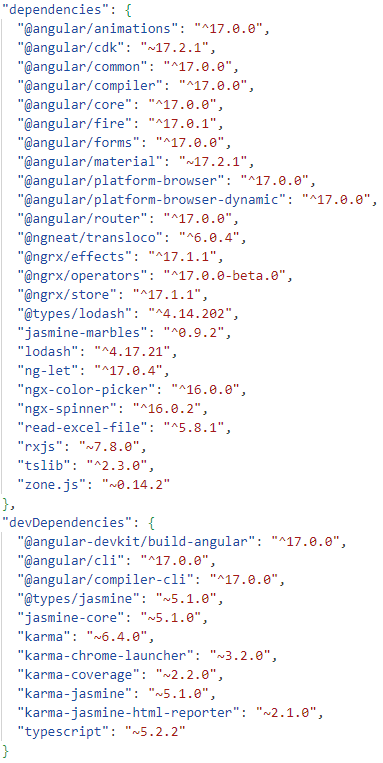
\includegraphics[width=0.45\linewidth]{dependencies.PNG}
    \caption{Az összes, az alkalmazáshoz felhasznált NPM csomag, részlet a package.json fájlból}
    \label{fig:dependencies}
\end{figure}

\begin{figure}[h]
    \centering
    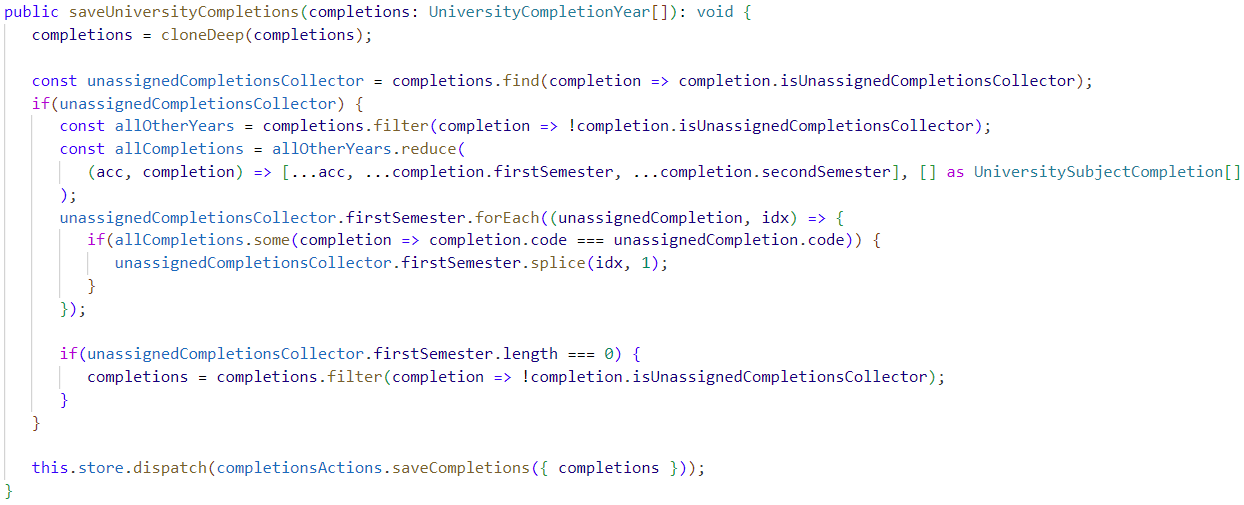
\includegraphics[width=1\linewidth]{adat_útvonal_04.PNG}
    \caption{Az elmentendő teljesítések módosítását és mentésre való továbbítását végző metódus}
    \label{fig:CompletionsService.saveUniversityCompletions}
\end{figure}

\begin{figure}[h]
    \centering
    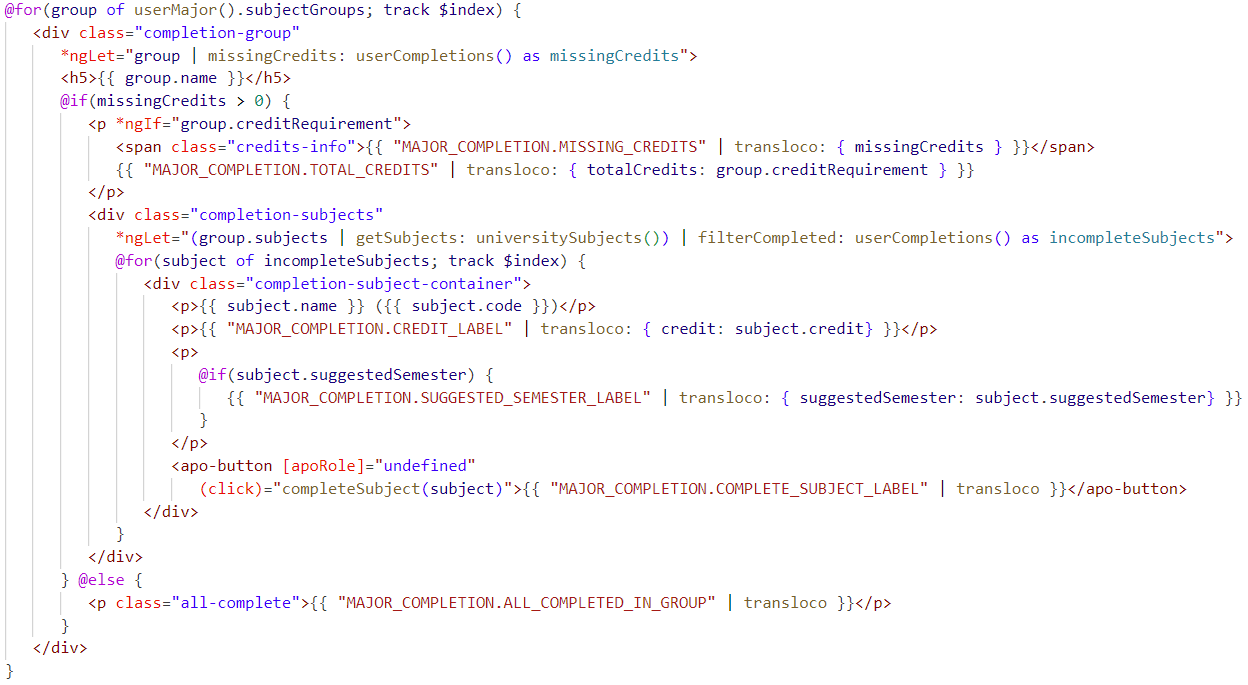
\includegraphics[width=1\linewidth]{adat_útvonal_09.PNG}
    \caption{A teljesítésekhez kapcsolódó adatokat megjelenítő HTML template}
    \label{fig:MajorCompletionComponentTemplate}
\end{figure}

\begin{figure}[h]
    \centering
    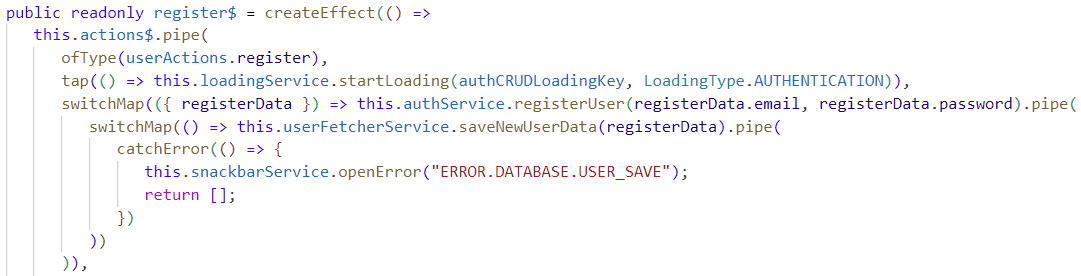
\includegraphics[width=0.75\linewidth]{regisztráció_1.PNG}
    \caption{A regisztrációt végző effect eleje, ami magát a regisztrációt végzi}
    \label{fig:UserEffectsRegister1}
\end{figure}

\begin{figure}[h]
    \centering
    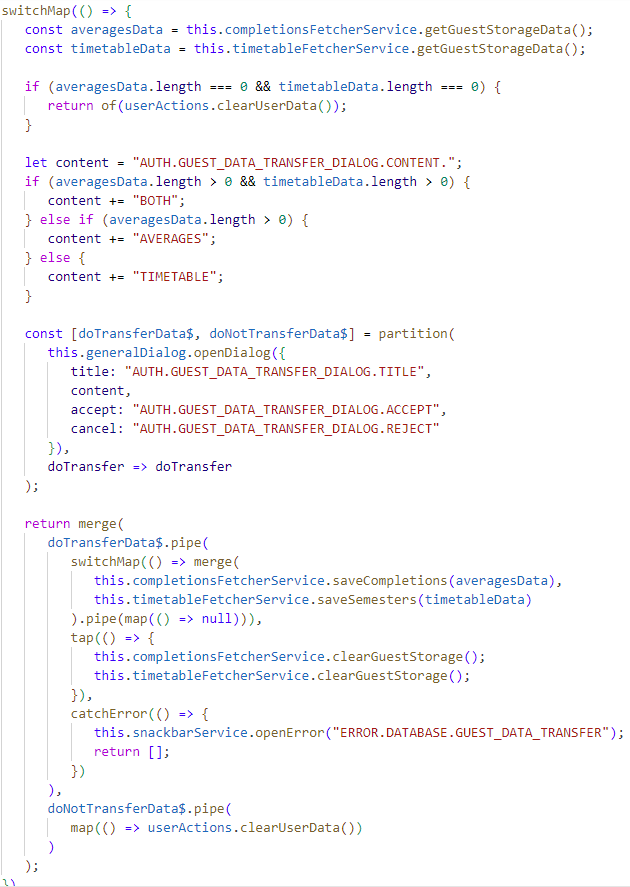
\includegraphics[width=0.75\linewidth]{regisztráció_2.PNG}
    \caption{A regisztrációt végző effect közepe, ami a vendégadatok átviteléért felelős}
    \label{fig:UserEffectsRegister2}
\end{figure}

\begin{figure}[h]
    \centering
    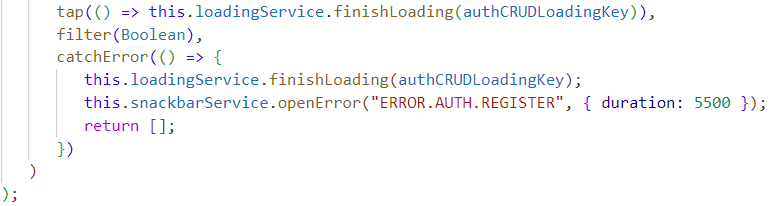
\includegraphics[width=0.75\linewidth]{regisztráció_3.PNG}
    \caption{A regisztrációt végző effect vége}
    \label{fig:UserEffectsRegister3}
\end{figure}

\begin{figure}[h]
    \centering
    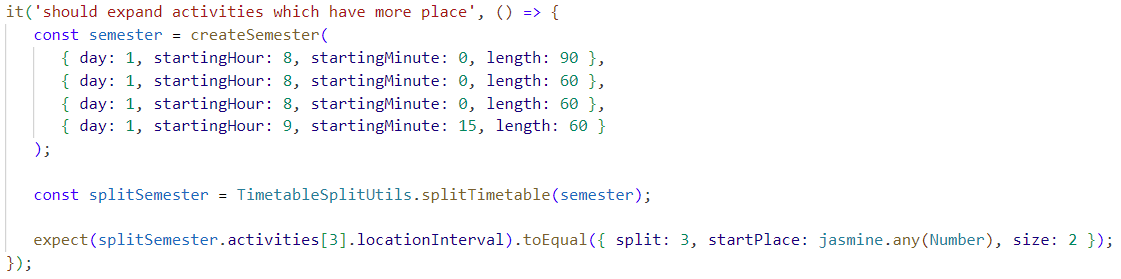
\includegraphics[width=1\linewidth]{órarend_teszt_2.PNG}
    \caption{A TimetableSplitUtils osztály egyik tesztesete egy jasmine segédfüggvénnyel}
    \label{fig:TimetableSplitUtilsTestJasmineAny}
\end{figure}

\begin{figure}[h]
    \centering
    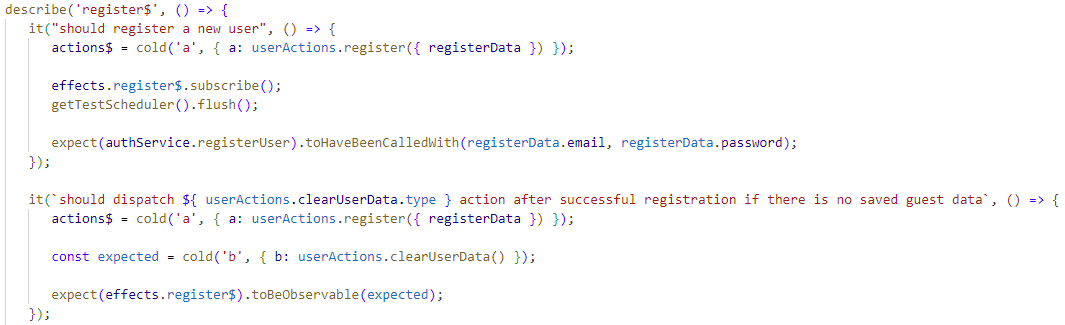
\includegraphics[width=1\linewidth]{regisztráció_teszt_3.PNG}
    \caption{A UserEffects regisztrációt ellenőrző néhány tesztje}
    \label{fig:UserEffectsSpecRegister}
\end{figure}

\end{document}
